\documentclass{article}

\usepackage{iclr2026_conference,times}
\usepackage[T1]{fontenc}
\usepackage[utf8]{inputenc}
\usepackage{microtype}
\usepackage{amsmath,amssymb}
\usepackage{booktabs}
\usepackage{tabularx}
\usepackage{array}
\usepackage{float}
\usepackage{graphicx}
\usepackage{xcolor}
\usepackage{tikz}
\usetikzlibrary{arrows.meta,positioning,shapes.geometric,fit}
\usepackage{hyperref}
\usepackage{url}

\definecolor{navy}{HTML}{173F73}
\definecolor{teal}{HTML}{138A8A}
\definecolor{orange}{HTML}{D97706}
\definecolor{rose}{HTML}{C23B53}
\definecolor{softgray}{HTML}{F1F4F8}
\definecolor{midgray}{HTML}{536274}

\hypersetup{
  colorlinks=true,
  linkcolor=navy,
  citecolor=teal,
  urlcolor=navy,
  pdftitle={Folding the Chain of Thought: Activation-Space Structure for Label-Free Reasoning Assessment},
  pdfauthor={Junjie Nian}
}

\newcommand{\nfs}{\textsc{NFS}}
\newcommand{\cotname}{CoT}
\newcommand{\repo}{\href{https://github.com/JunjieNian/cot_folding_demo}{public repository}}
\newcommand{\demo}{\href{http://demo.cot-folding.top}{interactive demo}}

\title{Folding the Chain of Thought:\\Activation-Space Structure for Label-Free Reasoning Assessment}

\author{Junjie Nian \\
College of Computer Science and Artificial Intelligence \\
Fudan University \\
Shanghai, China \\
\href{https://github.com/JunjieNian/cot_folding_demo}{\texttt{github.com/JunjieNian/cot\_folding\_demo}}}

\iclrfinalcopy

\begin{document}
\raggedbottom
\maketitle
\lhead{Preprint -- July 2026}

\begin{center}
\vspace{-0.7em}
\textbf{Live Demo:} \href{http://demo.cot-folding.top}{\texttt{demo.cot-folding.top}}
\end{center}
\vspace{0.3em}

\begin{abstract}
Long reasoning models can produce thousands of intermediate tokens, yet most evaluation reduces an entire trajectory to its final answer. Building on Neuron Agreement Decoding (NAD), this paper introduces \emph{CoT Folding}, a structural view of chain-of-thought reasoning in which fixed-length token slices are nodes and similarity between sparse neuron-activation signatures defines a contact geometry. A two-state hidden Markov model partitions the trajectory into exploration and exploitation phases. From the resulting graph we extract a dense backbone core, long-range return connections, unresolved drift branches, and final closure, then combine them into a label-free Native Fold Score (\nfs). On 1,920 AIME 2024 trajectories, \nfs{} separates correct from incorrect solutions with AUROC $0.7646$; aggregating HMM-contiguous segments raises AUROC to $0.8290$ and top-10\% selective accuracy to $99.48\%$. On 12,672 GPQA trajectories, slice-level \nfs{} reaches AUROC $0.6857$. Independent semantic checks show that activation-space similarity correlates with sentence-embedding similarity at mean Spearman $\rho=0.5704$, remains $0.5533$ after controlling for sequence distance, and collapses to approximately zero under paired shuffles. Across eleven reinforcement-learning checkpoints, the best label-free structural trend correlates with accuracy at $\rho=0.8273$, although it does not identify the exact best checkpoint. These results position CoT Folding as a diagnostic for structural coherence rather than a verifier of semantic truth: a confidently wrong trajectory can still fold well. We release the analysis pipeline, compact experimental artifacts, and an interactive visualization system.
\end{abstract}

\section{Introduction}

Chain-of-thought prompting and reasoning-oriented training have made long intermediate traces a routine part of language-model inference \citep{wei2022chain,wang2023selfconsistency,deepseek2025r1}. These traces expose useful process information, but they also create an evaluation mismatch. A final-answer label says whether a run succeeded, not whether its reasoning repeatedly returned to relevant subproblems, stabilized around a coherent plan, or drifted into a disconnected branch. Step-level supervision can recover some of this information, but it is expensive and task-dependent \citep{lightman2023verify}. Model confidence is cheaper, yet confidence alone can remain high for a coherent mistake \citep{kadavath2022know}.

We ask whether the \emph{geometry} of a reasoning trajectory contains a complementary signal. The motivating analogy is protein folding. A protein is a one-dimensional chain whose function depends on non-local contacts after folding; a reasoning trace is likewise sequential in text but can revisit an earlier quantity, reuse a sub-result, or return from exploration to a stable solution path. The analogy is operational rather than biological: we use it to define measurable contacts, cores, returns, and drift in activation space.

CoT Folding builds directly on Neuron Agreement Decoding (NAD), which represents generated chunks with sparse activated-neuron sets and measures cross-response consensus by Jaccard agreement \citep{chen2025nad}. Whereas NAD uses this signal for unsupervised best-of-$N$ response selection, we reuse its 32-token activation representation within a single response to study temporal folding. Every slice becomes a node; token entropy drives a two-state hidden Markov model (HMM) that labels slices as exploratory or exploitative. We then identify four structural primitives and combine them with a geometric mean. The result, \nfs, is label-free at scoring time and penalizes any trajectory missing a dense core, meaningful long-range return, or eventual closure.

The central empirical result is encouraging but deliberately limited. On AIME 2024 and GPQA, higher \nfs{} is associated with correctness and supports selective prediction. Segment-level aggregation improves the association. At the same time, high-scoring incorrect cases reveal that structural coherence is not semantic validity. Independent text encoders and shuffle controls further show that the activation contacts are not merely arbitrary geometry or token adjacency. Finally, checkpoint-level experiments suggest that structural trends can help monitor reinforcement learning without labels, while failing to resolve small non-monotonic accuracy differences.

Our contributions are threefold. First, we provide a graph representation of intra-trajectory reasoning built from sparse activation contacts and HMM phases. Second, we define an interpretable structural score and evaluate it across correctness discrimination, semantic alignment, and training dynamics. Third, we release an interactive system that links the geometry back to the original text, allowing aggregate scores to be audited slice by slice.

\begin{figure}[t]
\centering
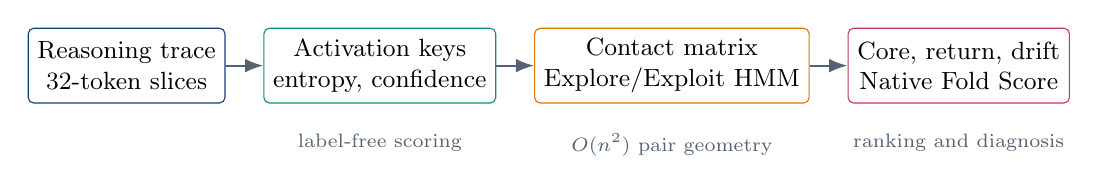
\begin{tikzpicture}[
  >=Latex,
  box/.style={draw, rounded corners=2pt, minimum width=2.35cm, minimum height=0.95cm, align=center, font=\small, fill=white},
  arrow/.style={->, thick, draw=midgray},
  note/.style={font=\scriptsize, text=midgray, align=center}
]
\node[box, draw=navy] (trace) {Reasoning trace\\32-token slices};
\node[box, draw=teal, right=0.48cm of trace] (signals) {Activation keys\\entropy, confidence};
\node[box, draw=orange, right=0.48cm of signals] (graph) {Contact matrix\\Explore/Exploit HMM};
\node[box, draw=rose, right=0.48cm of graph] (score) {Core, return, drift\\Native Fold Score};
\draw[arrow] (trace) -- (signals);
\draw[arrow] (signals) -- (graph);
\draw[arrow] (graph) -- (score);
\node[note, below=0.26cm of signals] {label-free scoring};
\node[note, below=0.26cm of graph] {$O(n^2)$ pair geometry};
\node[note, below=0.26cm of score] {ranking and diagnosis};
\end{tikzpicture}
\caption{CoT Folding converts a linear reasoning trace into an activation-space contact graph, extracts interpretable primitives, and produces a label-free structural score.}
\label{fig:pipeline}
\end{figure}

\section{Related Work}

\paragraph{Neuron Agreement Decoding.}
NAD finds that correct sampled responses tend to recruit more consistent neuron sets than incorrect ones and turns this observation into an unsupervised best-of-$N$ decoder \citep{chen2025nad}. CoT Folding adopts NAD's chunk-level activated-neuron representation and Jaccard geometry, but changes the unit of analysis from agreement among independently sampled responses to structural organization within one reasoning trajectory. This distinction is central: NAD selects among candidate answers, whereas our method diagnoses cores, returns, drift, and closure along a candidate's internal path.

\paragraph{Reasoning traces and verification.}
CoT prompting elicits explicit intermediate steps and improves multi-step reasoning in sufficiently capable models \citep{wei2022chain}. Self-consistency treats diverse reasoning paths as evidence by sampling multiple traces and aggregating their answers \citep{wang2023selfconsistency}. Reasoning-oriented reinforcement learning further encourages behaviors such as reflection and backtracking \citep{deepseek2025r1}. These gains do not make a trace a faithful account of the model's causal computation: plausible explanations can rationalize biased or incorrect answers \citep{turpin2023unfaithful}. Our method therefore does not interpret a well-folded path as proof that the verbalized reasoning is faithful.

Process reward models evaluate intermediate steps directly and can outperform outcome-only supervision, but require step-level judgments \citep{lightman2023verify}. Self-evaluation and calibrated confidence offer another route to failure prediction \citep{kadavath2022know}. CoT Folding instead asks whether a single trace has a coherent internal contact pattern. It is complementary to semantic verifiers because its score uses neither correctness labels nor an external judge at inference time.

\paragraph{Sequential state and geometry.}
HMMs provide a compact probabilistic model for segmenting observations into persistent latent states \citep{rabiner1989hmm}. We use a two-state Viterbi decoder as an operational partition between high-entropy exploration and low-entropy exploitation. Classical multidimensional scaling (MDS) embeds the pairwise distances for visualization \citep{torgerson1952mds}. The MDS coordinates are not used to compute \nfs; scoring occurs in the original pairwise geometry.

\paragraph{Selective prediction and semantic similarity.}
Selective prediction evaluates whether a score can trade coverage for lower risk \citep{geifman2017selective}. This is a natural test for a label-free reasoning-quality score. To validate that the activation geometry contains linguistic content, we compare it with TF--IDF, Sentence-BERT-style embeddings \citep{reimers2019sentencebert}, and a cross-encoder. These external text models validate an association between geometry and meaning; they are not components of \nfs.

\section{Method}

\subsection{From a token sequence to a contact graph}

Let a reasoning trajectory contain $T$ generated tokens. Following NAD \citep{chen2025nad}, we partition it into $n=\lceil T/32\rceil$ consecutive slices. For slice $i$, the activation cache provides a set $K_i$ of sparse neuron keys, together with token-level confidence and negative entropy. The structural similarity and distance are
\begin{equation}
s_{ij}=\frac{|K_i\cap K_j|}{|K_i\cup K_j|},
\qquad d_{ij}=1-s_{ij}.
\label{eq:jaccard}
\end{equation}
The full $n\times n$ matrix preserves long-range relations that would be discarded by a local chain or a small-window graph.

For the 32 tokens in slice $i$, confidence is averaged and entropy is computed as the negative mean cached negative-entropy plus $0.1$ times its within-slice standard deviation. A two-state Gaussian HMM uses the 75th and 25th entropy percentiles as initial emission means, half of the trajectory variance as each emission variance, and self-transition probability $p_{\mathrm{stay}}=0.9$. Viterbi decoding labels state 0 as \emph{exploration} and state 1 as \emph{exploitation}. This naming is descriptive: the HMM observes uncertainty, not the semantic role of a sentence.

We define a data-adaptive contact threshold
\begin{equation}
\tau=\operatorname{mean}_{i<j}(s_{ij})+\operatorname{std}_{i<j}(s_{ij}),
\end{equation}
and call a contact long-range when $|i-j|>\lfloor n/4\rfloor$. The same matrix supports optional 2D or 3D classical MDS views, contact maps, and contact-density plots.

\subsection{Structural primitives}

The score is built from four auditable primitives.

\paragraph{Backbone core.}
We split the exploitation states into contiguous blocks, seed the core with the largest block, and greedily merge another exploitation block when its mean similarity to the current core exceeds $\tau$. If $s_{\mathrm{core}}$ is mean within-core similarity and $f_{\mathrm{core}}$ is the fraction of all exploitation slices captured by the core, the backbone term is
\begin{equation}
B=s_{\mathrm{core}}f_{\mathrm{core}}.
\end{equation}

\paragraph{Long-range return.}
A return edge $e=(i,j)$ is a contact above $\tau$, spans more than $n/4$ slices, and has at least one exploitation endpoint. Its normalized contribution rewards both excess similarity and temporal span:
\begin{equation}
h_e=\frac{s_e-\tau}{1-\tau+\epsilon}\frac{g_e}{n-1},
\qquad H=\frac{1}{|E_r|}\sum_{e\in E_r}h_e,
\end{equation}
where $g_e=|i-j|$ and $H=0$ if no return edge exists.

\paragraph{Unresolved drift and closure.}
Each contiguous exploration branch $b$ has length $\ell_b$, normalized temporal midpoint $t_b$, and maximum similarity $m_b$ to the core. Its continuous unresolved fraction is $1-\min(1,m_b/\tau)$; later branches receive weight $w_b=1+t_b$. Thus
\begin{equation}
D_0=\frac{\sum_b w_b\ell_b\left(1-\min(1,m_b/\tau)\right)}{\sum_b w_b\ell_b}.
\end{equation}
Let $C=\min(1,s_{\mathrm{close}}/\tau)$ measure the maximum connection between the final exploitation block and the core. We use $G=(1+C)/2$ as a closure gate and define adjusted drift as $D^{\star}=1-G(1-D_0)$.

\subsection{Native Fold Score}

The final score is the geometric mean
\begin{equation}
\nfs=100\left[BH(1-D^{\star})\right]^{1/3}.
\label{eq:nfs}
\end{equation}
The multiplicative form encodes a strict design prior: a trajectory should not receive a high structural score by compensating for a missing core with many weak contacts, or by compensating for unresolved late drift with a dense local cluster. Although no labels enter Equation~\ref{eq:nfs}, the method has fixed construction choices such as slice length, $p_{\mathrm{stay}}$, and the contact rule; ``label-free'' should not be read as hyperparameter-free.

\subsection{Segment-level folding}

Slice-level graphs can overemphasize local noise. We therefore collapse adjacent slices with the same HMM state into segments and split segments longer than eight slices; high-variance segments can be divided at their largest internal dissimilarity. Two graph constructions are evaluated: \emph{union} computes Jaccard distance between the union of keys in each segment, while \emph{average} averages all cross-slice distances between two segments. The same primitives and geometric aggregation are then recomputed, with segment size carried into drift weighting.

\section{Experimental Setup}

\subsection{Datasets and model}

The main corpus contains 1,920 AIME 2024 trajectories: 30 competition problems with 64 sampled runs per problem. A second corpus contains 12,672 trajectories from the 198-question GPQA Diamond subset, again with 64 runs per question \citep{rein2024gpqa}. Both use DeepSeek-R1-0528-Qwen3-8B. Overall accuracies are 75.36\% on AIME and 60.17\% on GPQA. The AIME activation graph contains 883,462 slices and 264,073,064 undirected pairs. The recorded batch run completed in 1,877.5 seconds with approximately 1.46 GB incremental memory.

We also analyze eleven reinforcement-learning checkpoints of Qwen3-4B-Base, from the base model through step 1,000, on a variable-reasoning mathematics set. The checkpoint experiment asks whether statistics aggregated across all generations can rank training states without using per-sample correctness.

\subsection{Evaluation}

Correctness discrimination uses AUROC, AUPRC, Cohen's $d$, accuracy among the highest-scoring 10\% of trajectories, and Hit@1 within each problem. Selective accuracy measures whether abstaining on low-\nfs{} samples improves reliability, rather than treating \nfs{} as a calibrated probability.

Semantic validation compares the upper triangles of structural and text-similarity matrices within every AIME trajectory. Tier 1 uses TF--IDF cosine similarity. Tier 2 encodes each slice with \texttt{all-MiniLM-L6-v2}; the primary result is the per-trajectory Spearman correlation. We additionally partial out sequence distance, compare the five nearest structural neighbors with sequential and random neighbors, and independently shuffle either structure or text ten times. Tier 3 scores 5,000 structure-stratified slice pairs with \texttt{stsb-distilroberta-base}. Tier 4 uses cosine similarity over the source model's weighted sparse activations; because it shares a source with the structural keys, we treat it as an internal-consistency upper bound rather than independent validation.

\section{Results}

\subsection{Structural coherence predicts correctness}

Table~\ref{tab:discrimination} shows that \nfs{} consistently ranks correct trajectories above incorrect ones. On AIME, the mean gap is 2.62 points and AUROC is 0.7646; on GPQA, the gap is 2.31 points and AUROC is 0.6857. The top decile is substantially more accurate than the full sample on both tasks. Because AUPRC depends on prevalence, we report it together with the corresponding overall accuracy rather than comparing it across datasets in isolation.

\begin{table}[H]
\caption{Slice-level \nfs{} correctness discrimination. Mean scores are reported as mean $\pm$ standard deviation.}
\label{tab:discrimination}
\centering
\small
\setlength{\tabcolsep}{5pt}
\begin{tabular}{lcc}
\toprule
Metric & AIME 2024 & GPQA Diamond \\
\midrule
Trajectories & 1,920 & 12,672 \\
Overall accuracy & 75.36\% & 60.17\% \\
\nfs{} (correct) & $12.60\pm2.66$ & $12.72\pm3.82$ \\
\nfs{} (incorrect) & $9.98\pm3.16$ & $10.41\pm3.21$ \\
AUROC & \textbf{0.7646} & \textbf{0.6857} \\
AUPRC & 0.8784 & 0.7569 \\
Cohen's $d$ & 0.937 & 0.643 \\
Top-10\% accuracy & 92.19\% & 86.35\% \\
Hit@1 & 0.6667 & 0.6263 \\
\bottomrule
\end{tabular}
\end{table}

The two HMM phases are also statistically distinct in activation space. A Mann--Whitney test separates within-state from cross-state distance distributions for all 1,920 AIME trajectories and 12,500 of 12,672 GPQA trajectories (98.6\%). Mean distance separation is 0.0358 and 0.0277, respectively. The effect is consistent but modest, reinforcing that the labels describe a soft phase partition rather than two disconnected modes.

\subsection{Segments improve AIME ranking}

Aggregating coherent phases materially improves AIME discrimination (Table~\ref{tab:segments}). The average-distance segment graph reaches AUROC 0.8290, AUPRC 0.9295, and 99.48\% accuracy among the top-scoring tenth. It also raises per-problem Hit@1 from 0.6667 to 0.8000. The improvement supports the hypothesis that the relevant unit is often a phase rather than an arbitrary 32-token window.

\begin{table}[H]
\caption{AIME discrimination by graph granularity. Parentheses show AUROC gain over the slice baseline.}
\label{tab:segments}
\centering
\small
\begin{tabular}{lccc}
\toprule
Metric & Slice & Segment union & Segment average \\
\midrule
AUROC & 0.7646 & 0.7911 $(+0.027)$ & \textbf{0.8290} $(+0.064)$ \\
AUPRC & 0.8784 & 0.9091 & \textbf{0.9295} \\
Top-10\% accuracy & 92.19\% & 97.40\% & \textbf{99.48\%} \\
Hit@1 & 0.6667 & 0.7333 & \textbf{0.8000} \\
\bottomrule
\end{tabular}
\end{table}

\subsection{Activation contacts carry semantic information}

The structural matrix is strongly aligned with independent text representations. Mean per-trajectory Spearman correlation rises from 0.4542 for TF--IDF to 0.5704 for MiniLM sentence embeddings (Figure~\ref{fig:semantic}). A cross-encoder yields $\rho=0.7370$ on 5,000 stratified pairs. The same-source sparse representation reaches 0.8268, as expected from partially shared information, and is not counted as independent evidence.

\begin{figure}[t]
\centering
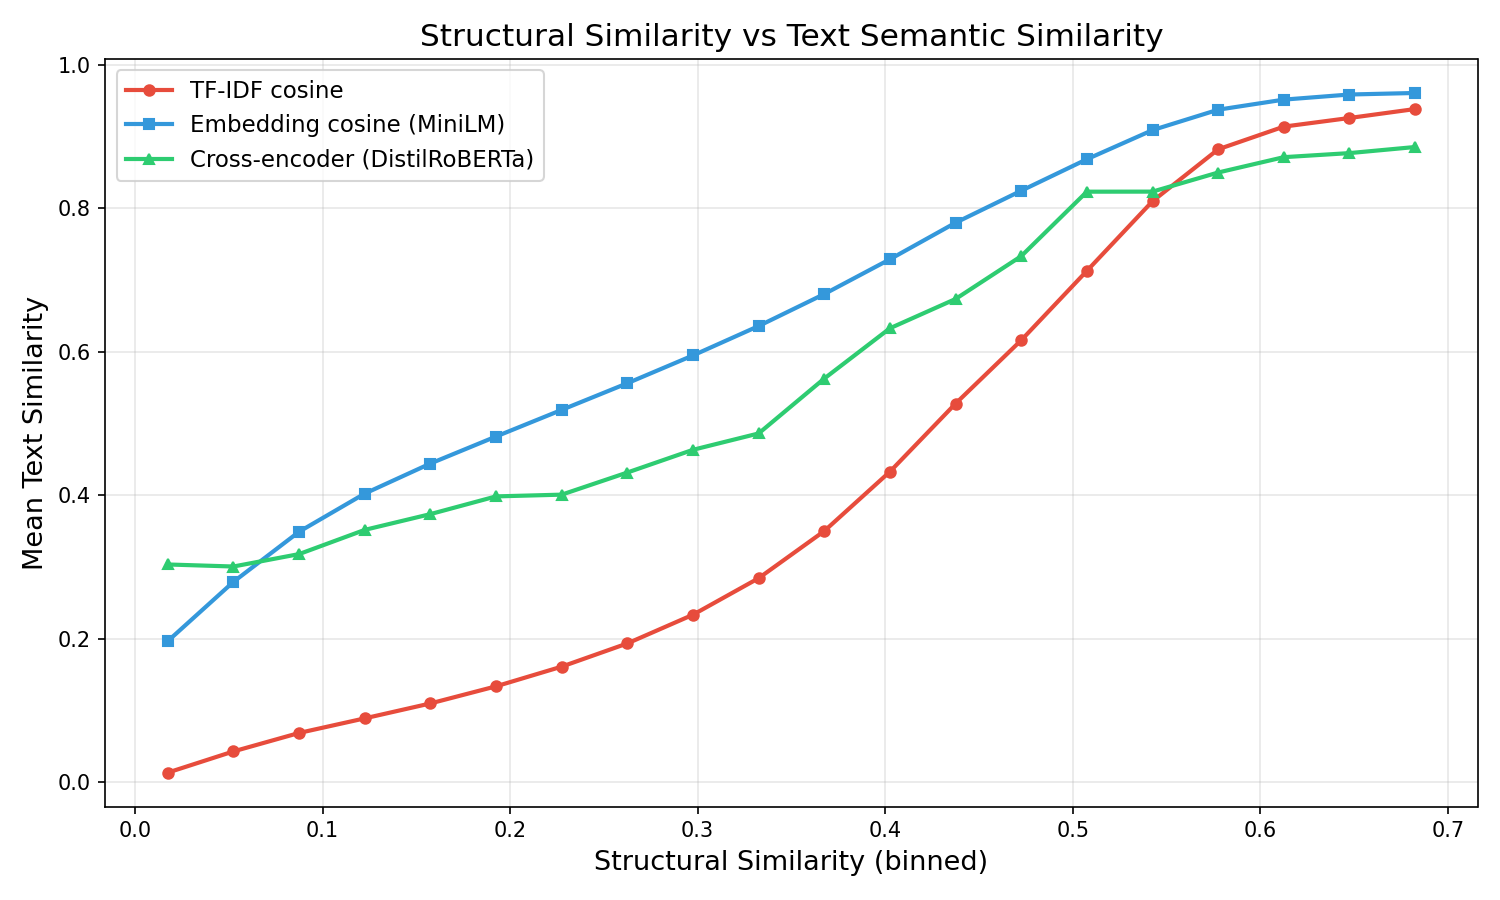
\includegraphics[width=\linewidth]{figures/semantic_alignment.png}
\caption{Binned activation-structure similarity versus three independent text-similarity measures. All three increase monotonically, although their scales are not directly comparable.}
\label{fig:semantic}
\end{figure}

\begin{table}[H]
\caption{Semantic validation on 1,920 AIME trajectories. Per-sample entries are means of Spearman correlations; the cross-encoder uses sampled pairs.}
\label{tab:semantic}
\centering
\small
\begin{tabularx}{\linewidth}{>{\raggedright\arraybackslash}Xrrl}
\toprule
Validation & $\rho$ & Units & Interpretation \\
\midrule
TF--IDF cosine & 0.4542 & 1,920 traces & lexical baseline \\
MiniLM embedding & 0.5704 & 1,920 traces & independent semantic test \\
Position-controlled & 0.5533 & 1,920 traces & sequence distance removed \\
Cross-encoder & 0.7370 & 5,000 pairs & stratified pair scoring \\
Source sparse cosine & 0.8268 & 1,920 traces & same-source upper bound \\
\bottomrule
\end{tabularx}
\end{table}

Position does not explain the association. After partialling out slice distance, mean $\rho$ decreases only from 0.5704 to 0.5533. The five nearest structural neighbors have mean MiniLM similarity 0.6601, compared with 0.5450 for sequentially adjacent slices and 0.3567 for random slices. Finally, independently permuting either the text order or structural order reduces mean correlation to 0.0003 and 0.0002, respectively, versus 0.5704 observed; all trajectories exceed the experiment's empirical significance threshold. Figure~\ref{fig:controls} displays both the raw/position-controlled distributions and the shuffle null.

\begin{figure}[H]
\centering
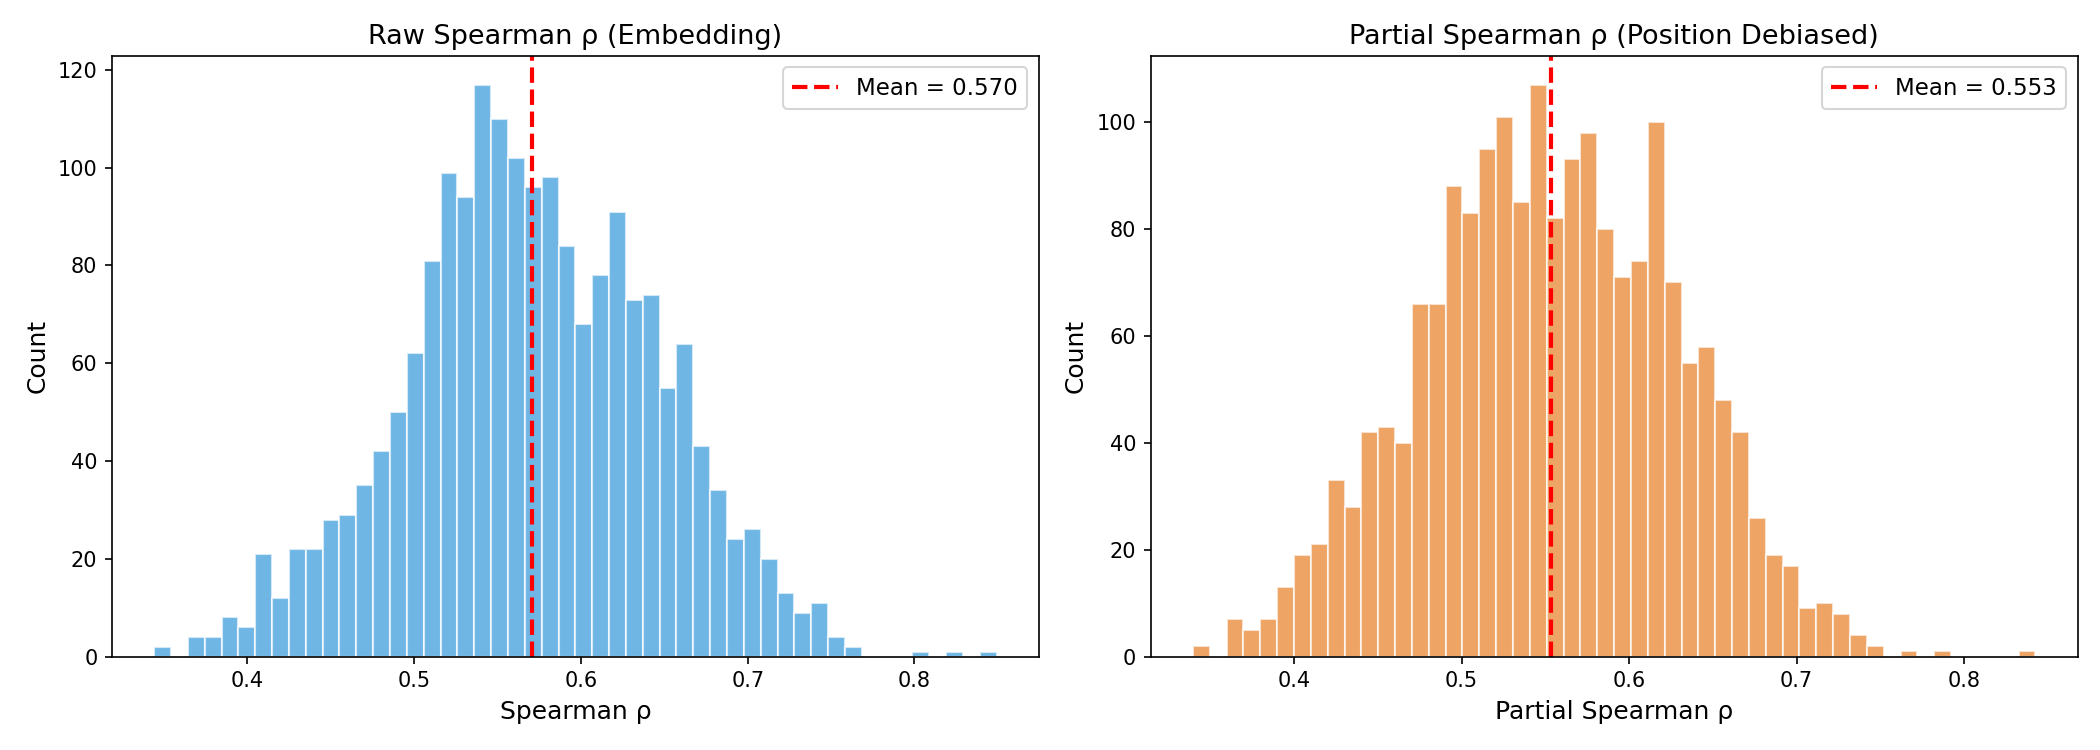
\includegraphics[width=\linewidth]{figures/position_control.png}
\caption{The distribution of per-trajectory structural--semantic correlations before (left) and after (right) controlling for sequence distance. The mean changes only from 0.570 to 0.553. Independent text and structure shuffles, reported in the paragraph above, reduce the mean association to approximately zero.}
\label{fig:controls}
\end{figure}

\subsection{A diagnostic, not a semantic verifier}

Case studies expose the score's boundary. A correct AIME trajectory with \nfs{} 15.83 forms a dense unified backbone with long-range return connections. An incorrect trajectory with \nfs{} 6.37 is fragmented and repeatedly drifts. Yet another incorrect trajectory scores 11.95 because it is internally consistent around a wrong intermediate value. The score detects fragmentation more directly than false premises or arithmetic errors. This distinction also explains why correct trajectories have slightly \emph{lower} mean structure--text correlation than incorrect ones (0.566 versus 0.583, Mann--Whitney $p=3.56\times10^{-6}$): semantic self-similarity within a trace is not synonymous with correctness.

\subsection{Label-free checkpoint monitoring is useful but imprecise}

Across eleven Qwen3-4B checkpoints, the ground-truth accuracy peaks at step 600 (33.19\%). The strongest label-free signal, the negative slope of \nfs{} against trajectory length, has Spearman $\rho=0.8273$ and Pearson $r=0.8868$ with checkpoint accuracy. Negative mean slice-level $H$ and $B$ reach $\rho=0.8091$ and $0.8000$, respectively, exceeding mean confidence ($\rho=0.7364$). However, no label-free method selects step 600 as top-1; most favor step 700 or 900. Structural monitoring captures the broad training trend but cannot reliably distinguish small non-monotonic differences such as 33.19\%, 32.99\%, and 32.11\% at steps 600--800.

\section{Interactive System}

The \demo{} turns each aggregate statistic into an inspectable object. Users can switch between AIME and reinforcement-learning data, select problems and sampled trajectories, color nodes by entropy, confidence, or HMM state, and compare 2D, 3D, split, global, and answer-tail views. A synchronized text pane maps visual slices back to the original reasoning. Additional views include contact maps, phase diagrams, structural comparisons, and batch-level distributions.

Figure~\ref{fig:demo} shows AIME problem 60, sample 0. The interface juxtaposes two projections of 168 slices with the source CoT and reports correctness, \nfs, and semantic-alignment statistics. The visualization is an audit surface rather than evidence for the score: all quantitative results are computed before MDS projection.

\begin{figure}[H]
\centering
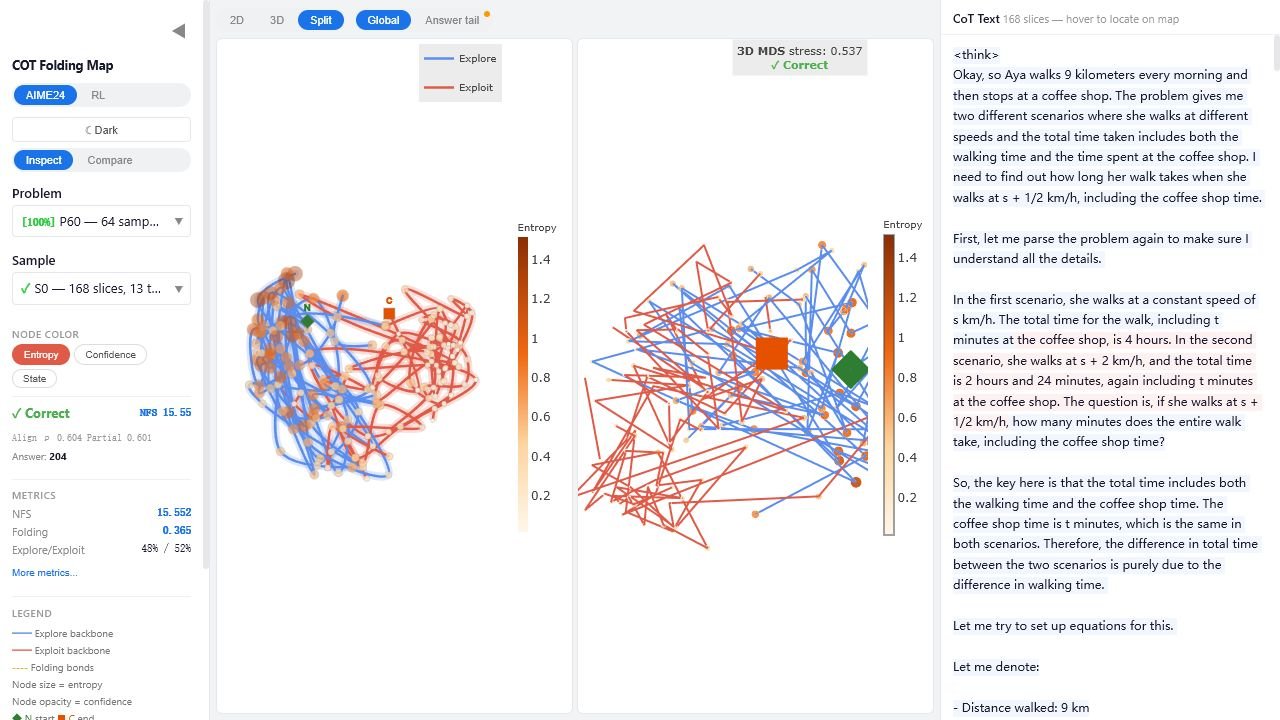
\includegraphics[width=\linewidth]{figures/demo_interface.png}
\caption{The released interactive demo. Explore and exploit backbones, entropy-colored nodes, endpoints, metrics, and the corresponding reasoning text are shown together. Screenshot captured from \url{http://demo.cot-folding.top}.}
\label{fig:demo}
\end{figure}

\section{Discussion}

The results support a narrow but useful claim: the internal trajectory geometry contains information about reasoning quality that is not reducible to token position or surface overlap. The strongest practical use is selective diagnosis. A high score can prioritize samples for answer aggregation or reduce the number of traces requiring external verification; a low score can point an analyst toward fragmentation, late drift, or a missing return to the main solution.

The protein-folding metaphor helps make those patterns legible, but it should not be reified. A neural activation contact is not a physical bond, and the HMM states are not cognitive states. Their value lies in the concrete operations they induce: non-local contact, persistent uncertainty phases, return-to-core strength, and closure. The semantic validation is therefore important. It demonstrates that the graph is related to meaning while leaving open which aspects of meaning the sparse keys capture.

Segment-level gains suggest that phase-aware compression is more than a visualization convenience. Arbitrary fixed windows introduce a resolution mismatch: a single mathematical subgoal may span several slices, whereas a long repetitive passage may occupy many nodes. Averaging cross-slice distances within HMM-contiguous segments reduces that mismatch. Future work should learn boundaries without correctness labels and test whether gains persist across slice widths, layers, architectures, and reasoning styles.

\section{Limitations}

\paragraph{Structural coherence is not truth.}
The central failure mode is a coherent but wrong derivation. \nfs{} must not be used as a correctness certificate or as a substitute for a verifier. The evaluation establishes ranking association, not logical validity.

\paragraph{Fixed design choices.}
The 32-token slice, $p_{\mathrm{stay}}=0.9$, mean-plus-standard-deviation contact threshold, and long-range cutoff $n/4$ are fixed heuristics. The score is label-free after these choices, not parameter-free. Robustness sweeps over each choice are needed.

\paragraph{Model and data scope.}
The main correctness experiments use one DeepSeek-R1-derived 8B model on mathematics and science benchmarks. GPQA is broader than AIME, but neither represents open-ended dialogue, code execution, multilingual reasoning, or tool use. The RL study uses only eleven checkpoints, so correlations are sensitive to individual points.

\paragraph{Activation dependence and circularity.}
Sparse activation keys depend on the upstream decomposition, selected model, and cached layer signals. Tier 4 is explicitly same-source and cannot validate semantic independence. Even Tiers 1--3 establish correlation, not that the graph recovers the model's causal computation.

\paragraph{Complexity and reproducibility.}
The full contact matrix costs $O(n^2)$ time and memory, making very long traces expensive. The repository releases source code and compact validation results, but not the large activation caches or every derived batch artifact. Exact regeneration therefore requires compatible upstream caches and model outputs.

\section{Ethics and Responsible Use}

Reasoning traces and activation caches can contain sensitive prompt content. Deployments should minimize retention, restrict access, and avoid publishing raw traces without permission. A structural score may also be tempting as an automated gate for models or people; the observed false-positive mode makes such use inappropriate without semantic verification and human review. The interactive interface is designed to expose the evidence behind a score rather than hide it behind a single number.

\section{Reproducibility Statement}

The \repo{} contains the slice- and segment-level graph builders, HMM implementation, primitive extraction, \nfs{} computation, RL checkpoint analysis, semantic-validation scripts, compact CSV/JSON summaries, generated plots, and the React visualization. Paths to external caches are configured through environment variables documented in the repository. The semantic artifacts record the sample counts and statistics reported here. Large NAD-style activation caches and derived distance matrices are excluded because of size. This manuscript source, bibliography, template files, and captured demo figure are included under \path{paper/}; the compiled artifact is written to \path{output/pdf/}.

\section{Conclusion}

CoT Folding provides a structural lens on long model reasoning. By transforming sparse activation signatures into contacts and combining a backbone, long-range returns, drift, and closure, \nfs{} ranks successful trajectories without consulting correctness labels at scoring time. Segment-level graphs improve AIME discrimination, independent text encoders validate semantic content in the geometry, and checkpoint trends show potential for training diagnostics. The same evidence also sets a clear boundary: good folding means coherent internal organization, not a true answer. The most promising next step is therefore hybrid evaluation in which structural diagnostics decide \emph{where} scrutiny is needed and semantic or executable verifiers decide \emph{whether} the reasoning is correct.

\bibliography{references}
\bibliographystyle{iclr2026_conference}

\appendix

\section{Native Fold Score Components}

\begin{table}[H]
\caption{Summary of the score components and their operational interpretation.}
\centering
\small
\begin{tabularx}{\linewidth}{cl>{\raggedright\arraybackslash}Xc}
\toprule
Symbol & Name & Definition & Range \\
\midrule
$B$ & Backbone & core internal similarity $\times$ covered exploit fraction & $[0,1]$ \\
$H$ & Return & mean normalized excess similarity $\times$ normalized gap & $[0,1]$ \\
$D_0$ & Drift & time- and length-weighted unresolved exploration & $[0,1]$ \\
$G$ & Gate & $(1+C)/2$ from final closure coefficient & $[0.5,1]$ \\
$D^{\star}$ & Adjusted drift & $1-G(1-D_0)$ & $[0,1]$ \\
\nfs & Fold score & $100[BH(1-D^{\star})]^{1/3}$ & $[0,100]$ \\
\bottomrule
\end{tabularx}
\end{table}

\section{Additional Terminal-Answer Analysis}

The repository includes an exploratory ``answer island'' analysis. A graph-based terminal-branch detector fires on 36.04\% of AIME trajectories and contains the extracted answer in 96.82\% of detected cases. A simpler HMM terminal-phase detector fires on 86.15\% and contains the answer in 98.00\%. The two detectors agree on 36.25\% of trajectories. These high conditional containment rates partly reflect that final answers occur near the end by construction; they should not be interpreted as evidence that the terminal phase caused correctness.

\begin{figure}[H]
\centering
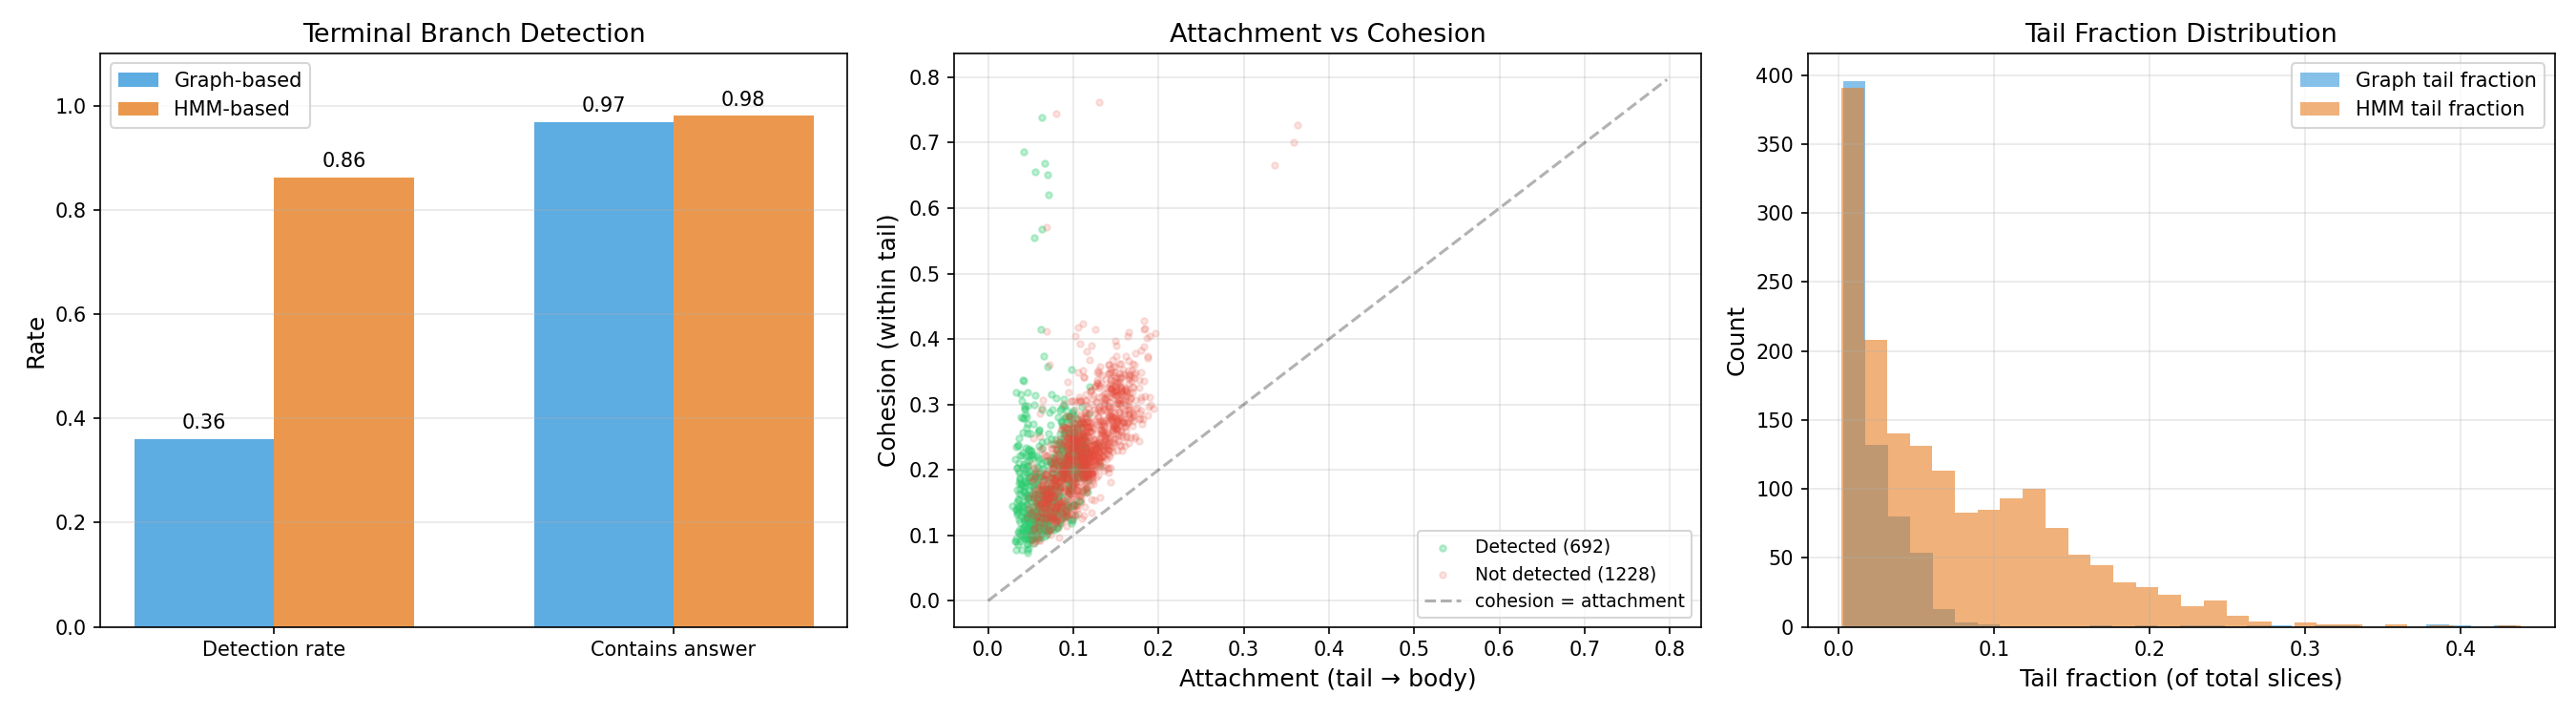
\includegraphics[width=0.92\linewidth]{figures/answer_island.png}
\caption{Exploratory terminal-answer analysis. Graph-based detection is selective, while the HMM tail is broad; both usually include the final answer when they fire.}
\end{figure}

\section{LLM Usage Disclosure}

AI writing and coding assistance was used to organize the manuscript, revise English prose, prepare LaTeX, and inspect the released repository and demo. Numerical results, formulas, and plots originate from the repository's tracked code, documentation, and compact result artifacts. The author remains responsible for verifying the experiments, interpretation, citations, and final manuscript.

\end{document}
